% Options for packages loaded elsewhere
\PassOptionsToPackage{unicode}{hyperref}
\PassOptionsToPackage{hyphens}{url}
%
\documentclass[
  ignorenonframetext,
]{beamer}
\usepackage{pgfpages}
\setbeamertemplate{caption}[numbered]
\setbeamertemplate{caption label separator}{: }
\setbeamercolor{caption name}{fg=normal text.fg}
\beamertemplatenavigationsymbolsempty
% Prevent slide breaks in the middle of a paragraph
\widowpenalties 1 10000
\raggedbottom
\setbeamertemplate{part page}{
  \centering
  \begin{beamercolorbox}[sep=16pt,center]{part title}
    \usebeamerfont{part title}\insertpart\par
  \end{beamercolorbox}
}
\setbeamertemplate{section page}{
  \centering
  \begin{beamercolorbox}[sep=12pt,center]{part title}
    \usebeamerfont{section title}\insertsection\par
  \end{beamercolorbox}
}
\setbeamertemplate{subsection page}{
  \centering
  \begin{beamercolorbox}[sep=8pt,center]{part title}
    \usebeamerfont{subsection title}\insertsubsection\par
  \end{beamercolorbox}
}
\AtBeginPart{
  \frame{\partpage}
}
\AtBeginSection{
  \ifbibliography
  \else
    \frame{\sectionpage}
  \fi
}
\AtBeginSubsection{
  \frame{\subsectionpage}
}
\usepackage{amsmath,amssymb}
\usepackage{iftex}
\ifPDFTeX
  \usepackage[T1]{fontenc}
  \usepackage[utf8]{inputenc}
  \usepackage{textcomp} % provide euro and other symbols
\else % if luatex or xetex
  \usepackage{unicode-math} % this also loads fontspec
  \defaultfontfeatures{Scale=MatchLowercase}
  \defaultfontfeatures[\rmfamily]{Ligatures=TeX,Scale=1}
\fi
\usepackage{lmodern}
\usetheme[]{Madrid}
\ifPDFTeX\else
  % xetex/luatex font selection
\fi
% Use upquote if available, for straight quotes in verbatim environments
\IfFileExists{upquote.sty}{\usepackage{upquote}}{}
\IfFileExists{microtype.sty}{% use microtype if available
  \usepackage[]{microtype}
  \UseMicrotypeSet[protrusion]{basicmath} % disable protrusion for tt fonts
}{}
\makeatletter
\@ifundefined{KOMAClassName}{% if non-KOMA class
  \IfFileExists{parskip.sty}{%
    \usepackage{parskip}
  }{% else
    \setlength{\parindent}{0pt}
    \setlength{\parskip}{6pt plus 2pt minus 1pt}}
}{% if KOMA class
  \KOMAoptions{parskip=half}}
\makeatother
\usepackage{xcolor}
\newif\ifbibliography
\usepackage{color}
\usepackage{fancyvrb}
\newcommand{\VerbBar}{|}
\newcommand{\VERB}{\Verb[commandchars=\\\{\}]}
\DefineVerbatimEnvironment{Highlighting}{Verbatim}{commandchars=\\\{\}}
% Add ',fontsize=\small' for more characters per line
\usepackage{framed}
\definecolor{shadecolor}{RGB}{248,248,248}
\newenvironment{Shaded}{\begin{snugshade}}{\end{snugshade}}
\newcommand{\AlertTok}[1]{\textcolor[rgb]{0.94,0.16,0.16}{#1}}
\newcommand{\AnnotationTok}[1]{\textcolor[rgb]{0.56,0.35,0.01}{\textbf{\textit{#1}}}}
\newcommand{\AttributeTok}[1]{\textcolor[rgb]{0.13,0.29,0.53}{#1}}
\newcommand{\BaseNTok}[1]{\textcolor[rgb]{0.00,0.00,0.81}{#1}}
\newcommand{\BuiltInTok}[1]{#1}
\newcommand{\CharTok}[1]{\textcolor[rgb]{0.31,0.60,0.02}{#1}}
\newcommand{\CommentTok}[1]{\textcolor[rgb]{0.56,0.35,0.01}{\textit{#1}}}
\newcommand{\CommentVarTok}[1]{\textcolor[rgb]{0.56,0.35,0.01}{\textbf{\textit{#1}}}}
\newcommand{\ConstantTok}[1]{\textcolor[rgb]{0.56,0.35,0.01}{#1}}
\newcommand{\ControlFlowTok}[1]{\textcolor[rgb]{0.13,0.29,0.53}{\textbf{#1}}}
\newcommand{\DataTypeTok}[1]{\textcolor[rgb]{0.13,0.29,0.53}{#1}}
\newcommand{\DecValTok}[1]{\textcolor[rgb]{0.00,0.00,0.81}{#1}}
\newcommand{\DocumentationTok}[1]{\textcolor[rgb]{0.56,0.35,0.01}{\textbf{\textit{#1}}}}
\newcommand{\ErrorTok}[1]{\textcolor[rgb]{0.64,0.00,0.00}{\textbf{#1}}}
\newcommand{\ExtensionTok}[1]{#1}
\newcommand{\FloatTok}[1]{\textcolor[rgb]{0.00,0.00,0.81}{#1}}
\newcommand{\FunctionTok}[1]{\textcolor[rgb]{0.13,0.29,0.53}{\textbf{#1}}}
\newcommand{\ImportTok}[1]{#1}
\newcommand{\InformationTok}[1]{\textcolor[rgb]{0.56,0.35,0.01}{\textbf{\textit{#1}}}}
\newcommand{\KeywordTok}[1]{\textcolor[rgb]{0.13,0.29,0.53}{\textbf{#1}}}
\newcommand{\NormalTok}[1]{#1}
\newcommand{\OperatorTok}[1]{\textcolor[rgb]{0.81,0.36,0.00}{\textbf{#1}}}
\newcommand{\OtherTok}[1]{\textcolor[rgb]{0.56,0.35,0.01}{#1}}
\newcommand{\PreprocessorTok}[1]{\textcolor[rgb]{0.56,0.35,0.01}{\textit{#1}}}
\newcommand{\RegionMarkerTok}[1]{#1}
\newcommand{\SpecialCharTok}[1]{\textcolor[rgb]{0.81,0.36,0.00}{\textbf{#1}}}
\newcommand{\SpecialStringTok}[1]{\textcolor[rgb]{0.31,0.60,0.02}{#1}}
\newcommand{\StringTok}[1]{\textcolor[rgb]{0.31,0.60,0.02}{#1}}
\newcommand{\VariableTok}[1]{\textcolor[rgb]{0.00,0.00,0.00}{#1}}
\newcommand{\VerbatimStringTok}[1]{\textcolor[rgb]{0.31,0.60,0.02}{#1}}
\newcommand{\WarningTok}[1]{\textcolor[rgb]{0.56,0.35,0.01}{\textbf{\textit{#1}}}}
\usepackage{graphicx}
\makeatletter
\def\maxwidth{\ifdim\Gin@nat@width>\linewidth\linewidth\else\Gin@nat@width\fi}
\def\maxheight{\ifdim\Gin@nat@height>\textheight\textheight\else\Gin@nat@height\fi}
\makeatother
% Scale images if necessary, so that they will not overflow the page
% margins by default, and it is still possible to overwrite the defaults
% using explicit options in \includegraphics[width, height, ...]{}
\setkeys{Gin}{width=\maxwidth,height=\maxheight,keepaspectratio}
% Set default figure placement to htbp
\makeatletter
\def\fps@figure{htbp}
\makeatother
\setlength{\emergencystretch}{3em} % prevent overfull lines
\providecommand{\tightlist}{%
  \setlength{\itemsep}{0pt}\setlength{\parskip}{0pt}}
\setcounter{secnumdepth}{-\maxdimen} % remove section numbering
\logo{
\includegraphics[height=1cm,width=3cm]{logo.png}}
\usetheme{Madrid}
\usefonttheme{serif}
\setbeamertemplate{navigation symbols}{}
\usepackage{lmodern}  % for bold teletype font
\usepackage{amsmath}  % for \hookrightarrow
\usepackage{xcolor}   % for \textcolor


\ifLuaTeX
  \usepackage{selnolig}  % disable illegal ligatures
\fi
\IfFileExists{bookmark.sty}{\usepackage{bookmark}}{\usepackage{hyperref}}
\IfFileExists{xurl.sty}{\usepackage{xurl}}{} % add URL line breaks if available
\urlstyle{same}
\hypersetup{
  pdftitle={Leksioni 5},
  pdfauthor={Endri Raco},
  hidelinks,
  pdfcreator={LaTeX via pandoc}}

\title{Leksioni 5}
\author{Endri Raco}
\date{01 May, 2024}

\begin{document}
\frame{\titlepage}

\begin{frame}[allowframebreaks]
  \tableofcontents[hideallsubsections]
\end{frame}
\hypertarget{puxebrgatitja-e-geodataframes-nga-tuxeb-dhuxebnat-gjeografike}{%
\section{Përgatitja e GeoDataFrames nga të dhënat
gjeografike}\label{puxebrgatitja-e-geodataframes-nga-tuxeb-dhuxebnat-gjeografike}}

\begin{frame}{Përgatitja e GeoDataFrames nga të dhënat gjeografike}
\protect\hypertarget{puxebrgatitja-e-geodataframes-nga-tuxeb-dhuxebnat-gjeografike-1}{}
\begin{itemize}
\item
  Leximi i të dhënave në Python është zakonisht hapi i parë i analizës.
\item
  Ekzistojnë formate të ndryshme të të dhënave GIS të disponueshme si
  \textbf{Shapefile, GeoJSON}, \textbf{KM} dhe \textbf{GeoPackage}.
\item
  \textbf{Geopandas} është në gjendje të lexojë të dhëna nga të gjitha
  këto formate (plus shumë të tjera).
\end{itemize}
\end{frame}

\begin{frame}{Përgatitja e GeoDataFrames nga të dhënat gjeografike}
\protect\hypertarget{puxebrgatitja-e-geodataframes-nga-tuxeb-dhuxebnat-gjeografike-2}{}
\begin{itemize}
\tightlist
\item
  Do shohim fillimisht se si të lexoni (dhe shkruani) të dhëna nga
  burime të ndryshme.
\end{itemize}
\end{frame}

\begin{frame}{Leximi i të dhënave vektoriale}
\protect\hypertarget{leximi-i-tuxeb-dhuxebnave-vektoriale}{}
\begin{itemize}
\item
  Në \textbf{geopandas}, ne mund të përdorim një funksion xhenerik
  \textbf{.from\_file()} për lexim në formate të ndryshme të të dhënave
  vektoriale.
\item
  Kur lexoni skedarë me gjeopanda, të dhënat kalohen në bibliotekën
  \textbf{fiona} në background.
\item
  Kjo do të thotë që ju mund të lexoni dhe shkruani të gjitha formatet e
  të dhënave të mbështetura nga \textbf{fiona} me \textbf{geopandas}.
\end{itemize}
\end{frame}

\begin{frame}[fragile]{Leximi i të dhënave vektoriale}
\protect\hypertarget{leximi-i-tuxeb-dhuxebnave-vektoriale-1}{}
\AddToHookNext{env/Highlighting/begin}{\scriptsize}

\begin{Shaded}
\begin{Highlighting}[]
\ImportTok{import}\NormalTok{ geopandas }\ImportTok{as}\NormalTok{ gpd}
\ImportTok{import}\NormalTok{ fiona}
\end{Highlighting}
\end{Shaded}
\end{frame}

\begin{frame}[fragile]{Leximi i të dhënave vektoriale}
\protect\hypertarget{leximi-i-tuxeb-dhuxebnave-vektoriale-2}{}
\begin{itemize}
\tightlist
\item
  Le të kontrollojmë se cilët drivera supportohen nga \textbf{fiona}.
\end{itemize}

\AddToHookNext{env/Highlighting/begin}{\scriptsize}

\begin{Shaded}
\begin{Highlighting}[]
\NormalTok{fiona.supported\_drivers}
\end{Highlighting}
\end{Shaded}

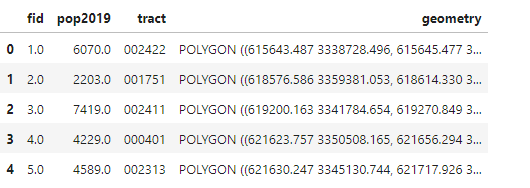
\includegraphics{./Figs/fiona1.png}
\end{frame}

\begin{frame}{Leximi i të dhënave vektoriale}
\protect\hypertarget{leximi-i-tuxeb-dhuxebnave-vektoriale-3}{}
\begin{itemize}
\item
  Në listën e drivera-ve të supportuar,\textbf{r} është për formatet e
  skedarëve që mund të lexojë fiona dhe \textbf{w} është për formatet e
  skedarëve që mund të shkruajë.
\item
  Shkronja \textbf{a} shënon formatet për të cilat fiona mund të shtojë
  të dhëna të reja në skedarët ekzistues.
\end{itemize}
\end{frame}

\begin{frame}[fragile]{Leximi i të dhënave vektoriale}
\protect\hypertarget{leximi-i-tuxeb-dhuxebnave-vektoriale-4}{}
\begin{itemize}
\tightlist
\item
  Le të lexojmë në disa të dhëna shembuj për të parë sintaksën bazë.
\end{itemize}

\AddToHookNext{env/Highlighting/begin}{\scriptsize}

\begin{Shaded}
\begin{Highlighting}[]
\CommentTok{\# Lexo nga Esri Shapefile}
\NormalTok{fp }\OperatorTok{=} \StringTok{"data/gis2/Austin/austin\_pop\_2019.shp"}
\NormalTok{data }\OperatorTok{=}\NormalTok{ gpd.read\_file(fp)}
\NormalTok{data.head()}
\end{Highlighting}
\end{Shaded}
\end{frame}

\begin{frame}{Leximi i të dhënave vektoriale}
\protect\hypertarget{leximi-i-tuxeb-dhuxebnave-vektoriale-5}{}
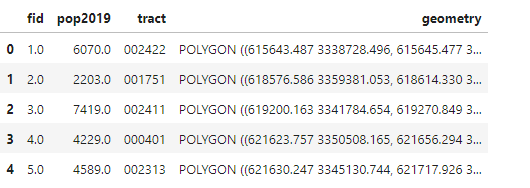
\includegraphics{./Figs/fiona1.png}
\end{frame}

\begin{frame}[fragile]{Leximi i të dhënave vektoriale}
\protect\hypertarget{leximi-i-tuxeb-dhuxebnave-vektoriale-6}{}
\begin{itemize}
\tightlist
\item
  E njëjta sintaksë funksionon për formate të tjera të të dhënave
  vektoriale të zakonshme.
\end{itemize}

\AddToHookNext{env/Highlighting/begin}{\scriptsize}

\begin{Shaded}
\begin{Highlighting}[]
\CommentTok{\# Lexo nga Geopackage}
\NormalTok{fp }\OperatorTok{=} \StringTok{"data/gis2/Austin/austin\_pop\_2019.gpkg"}
\NormalTok{data }\OperatorTok{=}\NormalTok{ gpd.read\_file(fp)}

\CommentTok{\# Lexo nga GeoJSON}
\NormalTok{fp }\OperatorTok{=} \StringTok{"data/gis2/Austin/austin\_pop\_2019.geojson"}
\NormalTok{data }\OperatorTok{=}\NormalTok{ gpd.read\_file(fp)}

\CommentTok{\# Lexo nga MapInfo Tab}
\NormalTok{fp }\OperatorTok{=} \StringTok{"data/gis2/Austin/austin\_pop\_2019.tab"}
\NormalTok{data }\OperatorTok{=}\NormalTok{ gpd.read\_file(fp)}
\end{Highlighting}
\end{Shaded}
\end{frame}

\begin{frame}{Leximi i të dhënave vektoriale}
\protect\hypertarget{leximi-i-tuxeb-dhuxebnave-vektoriale-7}{}
\begin{itemize}
\tightlist
\item
  Disa formate skedarësh si skedarët \textbf{GeoPackage} dhe
  \textbf{File Geodatabase} mund të përmbajnë shtresa të shumta me emra
  të ndryshëm, të cilët mund të specifikohen duke përdorur parametrin
  \textbf{layer}.
\end{itemize}
\end{frame}

\begin{frame}[fragile]{Leximi i të dhënave vektoriale}
\protect\hypertarget{leximi-i-tuxeb-dhuxebnave-vektoriale-8}{}
\AddToHookNext{env/Highlighting/begin}{\scriptsize}

\begin{Shaded}
\begin{Highlighting}[]
\CommentTok{\# Lexo nga GeoPackage }
\NormalTok{fp }\OperatorTok{=} \StringTok{"data/gis2/Austin/austin\_pop\_2019.gpkg"}
\NormalTok{data }\OperatorTok{=}\NormalTok{ gpd.read\_file(fp, layer}\OperatorTok{=}\StringTok{"austin\_pop\_2019"}\NormalTok{)}
\end{Highlighting}
\end{Shaded}
\end{frame}

\begin{frame}[fragile]{Leximi i të dhënave vektoriale}
\protect\hypertarget{leximi-i-tuxeb-dhuxebnave-vektoriale-9}{}
\AddToHookNext{env/Highlighting/begin}{\scriptsize}

\begin{Shaded}
\begin{Highlighting}[]
\CommentTok{\# Aktivizo KML driver}
\NormalTok{gpd.io.}\BuiltInTok{file}\NormalTok{.fiona.drvsupport.supported\_drivers[}\StringTok{"KML"}\NormalTok{] }\OperatorTok{=} \StringTok{"rw"}

\CommentTok{\# Lexo nga KML}
\NormalTok{fp }\OperatorTok{=} \StringTok{"data/gis2/Austin/austin\_pop\_2019.kml"}
\CommentTok{\# data = gpd.read\_file(fp)}
\end{Highlighting}
\end{Shaded}
\end{frame}

\begin{frame}{Shkrimi i të dhënave vektoriale}
\protect\hypertarget{shkrimi-i-tuxeb-dhuxebnave-vektoriale}{}
\begin{itemize}
\tightlist
\item
  Ne mund të ruajmë të dhëna hapësinore në formate të ndryshme të të
  dhënave vektoriale duke përdorur funksionin \textbf{.to\_file()} në
  \textbf{geopandas}, i cili gjithashtu mbështetet në \textbf{fiona}.
\end{itemize}
\end{frame}

\begin{frame}[fragile]{Shkrimi i të dhënave vektoriale}
\protect\hypertarget{shkrimi-i-tuxeb-dhuxebnave-vektoriale-1}{}
Krijoni folder \textbf{temp} brenda folderit \textbf{data}

\AddToHookNext{env/Highlighting/begin}{\scriptsize}

\begin{Shaded}
\begin{Highlighting}[]
\CommentTok{\# Shkruaj Shapefile (bëj kopje)}
\NormalTok{outfp }\OperatorTok{=} \StringTok{"data/temp/austin\_pop\_2019.shp"}
\NormalTok{data.to\_file(outfp)}

\CommentTok{\# Shkruaj Geopackage (bëj kopje)}
\NormalTok{outfp }\OperatorTok{=} \StringTok{"data/temp/austin\_pop\_2019.gpkg"}
\NormalTok{data.to\_file(outfp, driver}\OperatorTok{=}\StringTok{"GPKG"}\NormalTok{)}

\CommentTok{\# Shkruaj GeoJSON (bëj kopje)}
\NormalTok{outfp }\OperatorTok{=} \StringTok{"data/temp/austin\_pop\_2019.geojson"}
\NormalTok{data.to\_file(outfp, driver}\OperatorTok{=}\StringTok{"GeoJSON"}\NormalTok{)}

\CommentTok{\#Shkruaj MapInfo Tab (bëj kopje)}
\NormalTok{outfp }\OperatorTok{=} \StringTok{"data/temp/austin\_pop\_2019.tab"}
\NormalTok{data.to\_file(outfp)}


\CommentTok{\# Shkruaj KML (bëj kopje)}
\NormalTok{outfp }\OperatorTok{=} \StringTok{"data/temp/austin\_pop\_2019.kml"}
\NormalTok{data.to\_file(outfp, driver}\OperatorTok{=}\StringTok{"KML"}\NormalTok{)  }
\end{Highlighting}
\end{Shaded}
\end{frame}

\begin{frame}{Krijimi i një GeoDataFrame nga e para}
\protect\hypertarget{krijimi-i-njuxeb-geodataframe-nga-e-para}{}
\begin{itemize}
\item
  Është e mundur të krijohen të dhëna hapësinore nga e para duke
  përdorur objektet gjeometrike të \textbf{shapely} dhe
  \textbf{geopandas}.
\item
  Kjo është e dobishme pasi e bën të lehtë konvertimin, për shembull,
  një skedar teksti që përmban koordinata të të dhënave hapësinore.
\end{itemize}
\end{frame}

\begin{frame}{Krijimi i një GeoDataFrame nga e para}
\protect\hypertarget{krijimi-i-njuxeb-geodataframe-nga-e-para-1}{}
\begin{itemize}
\tightlist
\item
  Le të përpiqemi fillimisht të krijojmë një GeoDataFrame të thjeshtë
  bazuar në informacionin e koordinatave që përfaqësojnë skicat e
  sheshit të Senatit në Helsinki, Finlandë.
\end{itemize}
\end{frame}

\begin{frame}[fragile]{Krijimi i një GeoDataFrame nga e para}
\protect\hypertarget{krijimi-i-njuxeb-geodataframe-nga-e-para-2}{}
\begin{itemize}
\tightlist
\item
  Këtu janë koordinatat në bazë të të cilave mund të krijojmë një objekt
  Polygon duke përdorur `shapely.
\end{itemize}

\AddToHookNext{env/Highlighting/begin}{\scriptsize}

\begin{Shaded}
\begin{Highlighting}[]
\ImportTok{from}\NormalTok{ shapely.geometry }\ImportTok{import}\NormalTok{ Polygon}
\CommentTok{\# Koordinatat e sheshit të Senatit të Helsinkit}
\NormalTok{coordinates }\OperatorTok{=}\NormalTok{ [}
\NormalTok{    (}\FloatTok{24.950899}\NormalTok{, }\FloatTok{60.169158}\NormalTok{),}
\NormalTok{    (}\FloatTok{24.953492}\NormalTok{, }\FloatTok{60.169158}\NormalTok{),}
\NormalTok{    (}\FloatTok{24.953510}\NormalTok{, }\FloatTok{60.170104}\NormalTok{),}
\NormalTok{    (}\FloatTok{24.950958}\NormalTok{, }\FloatTok{60.169990}\NormalTok{),}
\NormalTok{]}

\CommentTok{\# Krijo një polygon Shapely nga lista e koordinatave{-}tuple}
\NormalTok{poly }\OperatorTok{=}\NormalTok{ Polygon(coordinates)}
\end{Highlighting}
\end{Shaded}
\end{frame}

\begin{frame}{Krijimi i një GeoDataFrame nga e para}
\protect\hypertarget{krijimi-i-njuxeb-geodataframe-nga-e-para-3}{}
\begin{itemize}
\item
  Tani mund ta përdorim këtë poligon dhe \textbf{geopanda} për të
  krijuar një GeoDataFrame nga e para.
\item
  Të dhënat mund të kalohen si një objekt i ngjashëm me listën.
\end{itemize}
\end{frame}

\begin{frame}{Krijimi i një GeoDataFrame nga e para}
\protect\hypertarget{krijimi-i-njuxeb-geodataframe-nga-e-para-4}{}
\begin{itemize}
\item
  Në rastin tonë do të kemi vetëm një rresht dhe një kolonë të dhënash.
\item
  Ne mund ta kalojmë poligonin brenda një liste dhe ta emërtojmë kolonën
  si \textbf{geometry} në mënyrë që \textbf{geopandas} të përdorin
  përmbajtjen e kolonës.
\end{itemize}
\end{frame}

\begin{frame}[fragile]{Krijimi i një GeoDataFrame nga e para}
\protect\hypertarget{krijimi-i-njuxeb-geodataframe-nga-e-para-5}{}
\AddToHookNext{env/Highlighting/begin}{\scriptsize}

\begin{Shaded}
\begin{Highlighting}[]
\NormalTok{newdata }\OperatorTok{=}\NormalTok{ gpd.GeoDataFrame(data}\OperatorTok{=}\NormalTok{[poly], columns}\OperatorTok{=}\NormalTok{[}\StringTok{"geometry"}\NormalTok{])}
\NormalTok{newdata}
\end{Highlighting}
\end{Shaded}
\end{frame}

\begin{frame}[fragile]{Krijimi i një GeoDataFrame nga e para}
\protect\hypertarget{krijimi-i-njuxeb-geodataframe-nga-e-para-6}{}
\AddToHookNext{env/Highlighting/begin}{\scriptsize}

\begin{Shaded}
\begin{Highlighting}[]
\CommentTok{\# Shto shtyllë dhe fut të dhëna}
\NormalTok{newdata.at[}\DecValTok{0}\NormalTok{, }\StringTok{"name"}\NormalTok{] }\OperatorTok{=} \StringTok{"Sheshi i Senatit"}

\CommentTok{\# Kontrollo}
\NormalTok{newdata}
\end{Highlighting}
\end{Shaded}
\end{frame}

\begin{frame}{Krijimi i një GeoDataFrame nga e para}
\protect\hypertarget{krijimi-i-njuxeb-geodataframe-nga-e-para-7}{}
\begin{itemize}
\item
  Tani kemi dy kolona në të dhënat tona; njëra që përfaqëson gjeometrinë
  dhe tjetra me informacion shtesë për atributet.
\item
  Nga këtu, mund të vazhdoni me shtimin e rreshtave shtesë të të dhënave
  ose printimin e të dhënave në një skedar.
\end{itemize}
\end{frame}

\begin{frame}{Krijimi i një GeoDataFrame nga një skedar teksti}
\protect\hypertarget{krijimi-i-njuxeb-geodataframe-nga-njuxeb-skedar-teksti}{}
\begin{itemize}
\item
  Një rast i zakonshëm është që të ketë koordinata në një
  \textbf{delimited textfile} që duhet të konvertohet në të dhëna
  hapësinore.
\item
  Për ta bërë këtë, ne mund të përdorim \textbf{pandas, geopandas} dhe
  \textbf{shapely}
\end{itemize}
\end{frame}

\begin{frame}[fragile]{Krijimi i një GeoDataFrame nga një skedar teksti}
\protect\hypertarget{krijimi-i-njuxeb-geodataframe-nga-njuxeb-skedar-teksti-1}{}
\AddToHookNext{env/Highlighting/begin}{\scriptsize}

\begin{Shaded}
\begin{Highlighting}[]
\ImportTok{import}\NormalTok{ pandas }\ImportTok{as}\NormalTok{ pd}
\NormalTok{airports }\OperatorTok{=}\NormalTok{ pd.read\_csv(}
    \StringTok{"data/gis2/Airports/airports.txt"}\NormalTok{,}
\NormalTok{    usecols}\OperatorTok{=}\NormalTok{[}\StringTok{"Airport ID"}\NormalTok{, }\StringTok{"Name"}\NormalTok{, }\StringTok{"City"}\NormalTok{, }\StringTok{"Country"}\NormalTok{, }\StringTok{"Latitude"}\NormalTok{, }\StringTok{"Longitude"}\NormalTok{],}
\NormalTok{)}
\NormalTok{airports.head()}
\end{Highlighting}
\end{Shaded}
\end{frame}

\begin{frame}{Krijimi i një GeoDataFrame nga një skedar teksti}
\protect\hypertarget{krijimi-i-njuxeb-geodataframe-nga-njuxeb-skedar-teksti-2}{}
\begin{itemize}
\tightlist
\item
  Të dhënat e shembullit përmbajnë koordinatat e pikave të aeroporteve
  që rrjedhin nga \textbf{openflights.org}.
\end{itemize}
\end{frame}

\begin{frame}[fragile]{Krijimi i një GeoDataFrame nga një skedar teksti}
\protect\hypertarget{krijimi-i-njuxeb-geodataframe-nga-njuxeb-skedar-teksti-3}{}
\AddToHookNext{env/Highlighting/begin}{\scriptsize}

\begin{Shaded}
\begin{Highlighting}[]
\BuiltInTok{len}\NormalTok{(airports)}
\end{Highlighting}
\end{Shaded}
\end{frame}

\begin{frame}{Krijimi i një GeoDataFrame nga një skedar teksti}
\protect\hypertarget{krijimi-i-njuxeb-geodataframe-nga-njuxeb-skedar-teksti-4}{}
\begin{itemize}
\item
  Ka mbi 7000 aeroporte në të dhënat dhe ne mund të përdorim
  informacionin e koordinatave të disponueshme në kolonat
  \textbf{Latitude} dhe \textbf{Longitude} për t'i vizualizuar ato në
  një hartë.
\item
  Koordinatat ruhen si gradë dhjetore, që do të thotë se sistemi i duhur
  i referencës së koordinatave për këto të dhëna është \textbf{WGS 84
  (EPSG:4326)}.
\end{itemize}
\end{frame}

\begin{frame}{Krijimi i një GeoDataFrame nga një skedar teksti}
\protect\hypertarget{krijimi-i-njuxeb-geodataframe-nga-njuxeb-skedar-teksti-5}{}
\begin{itemize}
\item
  Ekziston një metodë e dobishme në \textbf{geopandas} për gjenerimin e
  një grupi objektesh pikash bazuar në koordinatat x dhe y të quajtur
  \textbf{.points\_from\_xy()}.
\item
  Metoda supozon se koordinatat x përfaqësojnë gjatësinë dhe se
  koordinatat y përfaqësojnë gjerësinë gjeografike.
\end{itemize}
\end{frame}

\begin{frame}[fragile]{Krijimi i një GeoDataFrame nga një skedar teksti}
\protect\hypertarget{krijimi-i-njuxeb-geodataframe-nga-njuxeb-skedar-teksti-6}{}
\AddToHookNext{env/Highlighting/begin}{\scriptsize}

\begin{Shaded}
\begin{Highlighting}[]
\NormalTok{airports[}\StringTok{"geometry"}\NormalTok{] }\OperatorTok{=}\NormalTok{ gpd.points\_from\_xy(}
\NormalTok{    x}\OperatorTok{=}\NormalTok{airports[}\StringTok{"Longitude"}\NormalTok{], y}\OperatorTok{=}\NormalTok{airports[}\StringTok{"Latitude"}\NormalTok{], crs}\OperatorTok{=}\StringTok{"EPSG:4326"}
\NormalTok{)}

\NormalTok{airports }\OperatorTok{=}\NormalTok{ gpd.GeoDataFrame(airports)}
\NormalTok{airports.head()}
\end{Highlighting}
\end{Shaded}
\end{frame}

\begin{frame}[fragile]{Krijimi i një GeoDataFrame nga një skedar teksti}
\protect\hypertarget{krijimi-i-njuxeb-geodataframe-nga-njuxeb-skedar-teksti-7}{}
\begin{itemize}
\tightlist
\item
  Tani gjeometritë e pikave i kemi si \textbf{shapelyobjects} në kolonën
  \textbf{geometry} gati për t'u paraqitur në një hartë.
\end{itemize}

\AddToHookNext{env/Highlighting/begin}{\scriptsize}

\begin{Shaded}
\begin{Highlighting}[]
\NormalTok{airports.plot(markersize}\OperatorTok{=}\FloatTok{0.1}\NormalTok{)}
\end{Highlighting}
\end{Shaded}
\end{frame}

\begin{frame}{Krijimi i një GeoDataFrame nga një skedar teksti}
\protect\hypertarget{krijimi-i-njuxeb-geodataframe-nga-njuxeb-skedar-teksti-8}{}
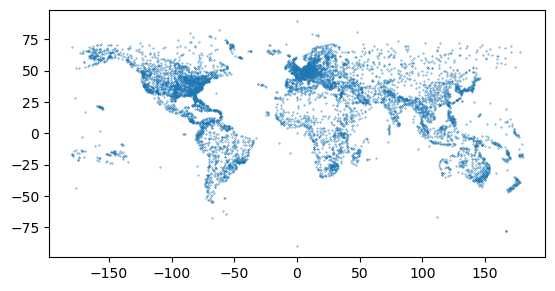
\includegraphics{./Figs/airports.png}
\end{frame}

\hypertarget{manipulimi-i-tuxeb-dhuxebnave-gjeometrike}{%
\section{Manipulimi i të dhënave
gjeometrike}\label{manipulimi-i-tuxeb-dhuxebnave-gjeometrike}}

\begin{frame}{Manipulimi i të dhënave gjeometrike}
\protect\hypertarget{manipulimi-i-tuxeb-dhuxebnave-gjeometrike-1}{}
\begin{itemize}
\item
  Do shohim disa nga funksionet më të zakonshme të manipulimit të
  gjeometrisë në \textbf{geopandas}.
\item
  Do të eksplorojmë të dhënat e censusit nga Austin, Teksas.
\end{itemize}
\end{frame}

\begin{frame}{Manipulimi i të dhënave gjeometrike}
\protect\hypertarget{manipulimi-i-tuxeb-dhuxebnave-gjeometrike-2}{}
\begin{itemize}
\tightlist
\item
  Shpesh është e dobishme të bëhen manipulime gjeometrike në kufijtë
  administrativë për qëllime të mëtejshme analize dhe vizualizimi.
\end{itemize}
\end{frame}

\begin{frame}[fragile]{Manipulimi i të dhënave gjeometrike}
\protect\hypertarget{manipulimi-i-tuxeb-dhuxebnave-gjeometrike-3}{}
\AddToHookNext{env/Highlighting/begin}{\scriptsize}

\begin{Shaded}
\begin{Highlighting}[]
\ImportTok{import}\NormalTok{ geopandas }\ImportTok{as}\NormalTok{ gpd}
\ImportTok{import}\NormalTok{ matplotlib.pyplot }\ImportTok{as}\NormalTok{ plt}
\ImportTok{from}\NormalTok{ pathlib }\ImportTok{import}\NormalTok{ Path}
\end{Highlighting}
\end{Shaded}
\end{frame}

\begin{frame}[fragile]{Manipulimi i të dhënave gjeometrike}
\protect\hypertarget{manipulimi-i-tuxeb-dhuxebnave-gjeometrike-4}{}
\AddToHookNext{env/Highlighting/begin}{\scriptsize}

\begin{Shaded}
\begin{Highlighting}[]
\NormalTok{fp }\OperatorTok{=} \StringTok{"data/gis2/Austin/austin\_pop\_2019.gpkg"}

\NormalTok{data }\OperatorTok{=}\NormalTok{ gpd.read\_file(fp)}
\NormalTok{data.head()}
\end{Highlighting}
\end{Shaded}
\end{frame}

\begin{frame}{Manipulimi i të dhënave gjeometrike}
\protect\hypertarget{manipulimi-i-tuxeb-dhuxebnave-gjeometrike-5}{}
\begin{itemize}
\item
  Për manipulime gjeometrike, ne jemi të interesuar kryesisht në kolonën
  \textbf{geometry} e cila përmban gjeometritë e poligonit.
\item
  Lloji i të dhënave të kolonës-gjeometri është \textbf{GeoSeries}.
\item
  Gjeometritë individuale janë objekte \textbf{shapely} dhe ne mund të
  përdorim të gjitha mjetet e \textbf{shapely} për manipulimin e
  gjeometrisë.
\end{itemize}
\end{frame}

\begin{frame}[fragile]{Manipulimi i të dhënave gjeometrike}
\protect\hypertarget{manipulimi-i-tuxeb-dhuxebnave-gjeometrike-6}{}
\AddToHookNext{env/Highlighting/begin}{\scriptsize}

\begin{Shaded}
\begin{Highlighting}[]
\CommentTok{\# Kontrollojmë kolonen geometry}
\NormalTok{data[}\StringTok{"geometry"}\NormalTok{].head()}
\end{Highlighting}
\end{Shaded}
\end{frame}

\begin{frame}[fragile]{Manipulimi i të dhënave gjeometrike}
\protect\hypertarget{manipulimi-i-tuxeb-dhuxebnave-gjeometrike-7}{}
\AddToHookNext{env/Highlighting/begin}{\scriptsize}

\begin{Shaded}
\begin{Highlighting}[]
\CommentTok{\# Kontrollojmë përmbajtjen}
\NormalTok{data[}\StringTok{"geometry"}\NormalTok{].head()}
\end{Highlighting}
\end{Shaded}
\end{frame}

\begin{frame}[fragile]{Manipulimi i të dhënave gjeometrike}
\protect\hypertarget{manipulimi-i-tuxeb-dhuxebnave-gjeometrike-8}{}
\AddToHookNext{env/Highlighting/begin}{\scriptsize}

\begin{Shaded}
\begin{Highlighting}[]
\CommentTok{\# Kontrollojmë tipin e te dhenave}
\BuiltInTok{type}\NormalTok{(data[}\StringTok{"geometry"}\NormalTok{].values[}\DecValTok{0}\NormalTok{])}
\end{Highlighting}
\end{Shaded}
\end{frame}

\begin{frame}[fragile]{Manipulimi i të dhënave gjeometrike}
\protect\hypertarget{manipulimi-i-tuxeb-dhuxebnave-gjeometrike-9}{}
\begin{itemize}
\tightlist
\item
  Le të paraqesim së pari gjeometritë origjinale.
\end{itemize}

\AddToHookNext{env/Highlighting/begin}{\scriptsize}

\begin{Shaded}
\begin{Highlighting}[]
\NormalTok{data.plot(facecolor}\OperatorTok{=}\StringTok{"none"}\NormalTok{, linewidth}\OperatorTok{=}\FloatTok{0.2}\NormalTok{)}

\NormalTok{plt.axis(}\StringTok{"off"}\NormalTok{)}
\NormalTok{plt.show()}
\end{Highlighting}
\end{Shaded}
\end{frame}

\begin{frame}{Centroidet}
\protect\hypertarget{centroidet}{}
\begin{itemize}
\item
  Nxjerrja e centroidit të karakteristikave gjeometrike është e dobishme
  në shumë raste.
\item
  Centroidi gjeometrik mund të përdoret, për shembull, për të vendosur
  etiketat e tekstit në vizualizime.
\end{itemize}
\end{frame}

\begin{frame}{Centroidet}
\protect\hypertarget{centroidet-1}{}
\begin{itemize}
\item
  Ne mund të nxjerrim pikën qendrore të çdo poligoni nëpërmjet
  atributeve të centroidit në kolonën gjeometri.
\item
  Të dhënat duhet të jenë në një sistem referencash të koordinatave të
  projektuar kur llogariten centroidet.
\end{itemize}
\end{frame}

\begin{frame}{Centroidet}
\protect\hypertarget{centroidet-2}{}
\begin{itemize}
\tightlist
\item
  Nëse përpiqeni të llogaritni centroidet bazuar në informacionin e
  gjerësisë dhe gjatësisë, \textbf{geopandas} do të na paralajmërojë se
  rezultatet ka shumë mundësi të jenë të pasakta.
\end{itemize}
\end{frame}

\begin{frame}{Centroidet}
\protect\hypertarget{centroidet-3}{}
\begin{itemize}
\tightlist
\item
  Të dhënat tona janë në \emph{WGS 84 / UTM zona 14N (EPSG:32614)}
\end{itemize}
\end{frame}

\begin{frame}[fragile]{Centroidet}
\protect\hypertarget{centroidet-4}{}
\AddToHookNext{env/Highlighting/begin}{\scriptsize}

\begin{Shaded}
\begin{Highlighting}[]
\NormalTok{data.crs.name}
\end{Highlighting}
\end{Shaded}
\end{frame}

\begin{frame}[fragile]{Centroidet}
\protect\hypertarget{centroidet-5}{}
\AddToHookNext{env/Highlighting/begin}{\scriptsize}

\begin{Shaded}
\begin{Highlighting}[]
\NormalTok{data[}\StringTok{"geometry"}\NormalTok{].centroid.head()}
\end{Highlighting}
\end{Shaded}
\end{frame}

\begin{frame}[fragile]{Centroidet}
\protect\hypertarget{centroidet-6}{}
\AddToHookNext{env/Highlighting/begin}{\scriptsize}

\begin{Shaded}
\begin{Highlighting}[]
\NormalTok{data.centroid.plot(markersize}\OperatorTok{=}\DecValTok{1}\NormalTok{)}

\NormalTok{plt.axis(}\StringTok{"off"}\NormalTok{)}
\NormalTok{plt.show()}
\end{Highlighting}
\end{Shaded}
\end{frame}

\begin{frame}[fragile]{Bashkimi Unar (Unary Union)}
\protect\hypertarget{bashkimi-unar-unary-union}{}
\begin{itemize}
\item
  Ne mund të gjenerojmë një vijë të përbashkët të zonave administrative
  duke krijuar një bashkim gjeometrik midis të gjitha gjeometrive.
\item
  Kjo mund të jetë e dobishme, për shembull, për të vizualizuar vijat e
  jashtme të një zone studimi.
\item
  \texttt{unary\_union} kthen një objekt të vetëm të tipit gjeometri, i
  cili vizualizohet automatikisht kur ekzekutoni kodin në një Jupyter
  Notebook.
\end{itemize}
\end{frame}

\begin{frame}[fragile]{Bashkimi Unar (Unary Union)}
\protect\hypertarget{bashkimi-unar-unary-union-1}{}
\AddToHookNext{env/Highlighting/begin}{\scriptsize}

\begin{Shaded}
\begin{Highlighting}[]
\CommentTok{\# Kryen bashkimin unar të të gjitha gjeometrive dhe kthen një objekt të vetëm të tipit gjeometri}
\NormalTok{data.unary\_union}
\end{Highlighting}
\end{Shaded}
\end{frame}

\begin{frame}[fragile]{Thjeshtëzimi i Gjeometrive}
\protect\hypertarget{thjeshtuxebzimi-i-gjeometrive}{}
\begin{itemize}
\item
  Simplifikimi i gjeometrisë është një proces i dobishëm sidomos kur
  vizualizoni të dhëna që kanë gjeometri shumë të detajuar.
\item
  Me të dhënat tona të mostrës, ne mund të gjenerojmë një version të
  thjeshtuar të përmasave të jashtme.
\item
  Parametri \texttt{tolerance} kontrollon nivelin e thjeshtimit.
\end{itemize}
\end{frame}

\begin{frame}[fragile]{Thjeshtëzimi i Gjeometrive}
\protect\hypertarget{thjeshtuxebzimi-i-gjeometrive-1}{}
\AddToHookNext{env/Highlighting/begin}{\scriptsize}

\begin{Shaded}
\begin{Highlighting}[]
\CommentTok{\# Kryen thjeshtimin e gjeometrisë me një nivel tolerance prej 1000 njësi}
\NormalTok{data.unary\_union.simplify(tolerance }\OperatorTok{=} \DecValTok{1000}\NormalTok{)}
\end{Highlighting}
\end{Shaded}
\end{frame}

\begin{frame}{Poligoni Kufizues}
\protect\hypertarget{poligoni-kufizues}{}
\begin{itemize}
\item
  Poligonët kufizues janë të dobishëm në shumë raste për të përshkruar
  përmasat e përafërta të të dhënave gjeografike.
\item
  Një drejtkëndësh minimal kufizues, i quajtur gjithashtu një kuti
  kufizuese ose zarf, është poligoni drejtkëndësh më i vogël që rrethon
  një objekt gjeometrik.
\end{itemize}
\end{frame}

\begin{frame}[fragile]{Poligoni Kufizues}
\protect\hypertarget{poligoni-kufizues-1}{}
Në një \texttt{GeoDataFrame}, atributi \texttt{envelope} kthen
drejtkëndëshin kufizues për çdo gjeometri.

\AddToHookNext{env/Highlighting/begin}{\scriptsize}

\begin{Shaded}
\begin{Highlighting}[]
\CommentTok{\# Merr drejtkëndëshin kufizues për çdo gjeometri dhe shfaq vetëm pesë të parat}
\NormalTok{data.envelope.head()}
\end{Highlighting}
\end{Shaded}
\end{frame}

\begin{frame}{Poligoni Kufizues}
\protect\hypertarget{poligoni-kufizues-2}{}
\begin{itemize}
\tightlist
\item
  Për të marrë drejtkëndëshin kufizues për të gjithë shtresën, ne së
  pari krijojmë një bashkim të të gjitha gjeometrive duke përdorur
  \textbf{unary\_union}, dhe më pas krijojmë drejtkëndëshin kufizues për
  atë poligon.
\end{itemize}
\end{frame}

\begin{frame}[fragile]{Poligoni Kufizues}
\protect\hypertarget{poligoni-kufizues-3}{}
\AddToHookNext{env/Highlighting/begin}{\scriptsize}

\begin{Shaded}
\begin{Highlighting}[]
\CommentTok{\# Merr drejtkëndëshin kufizues për të gjitha gjeometrinë}
\NormalTok{data.unary\_union.envelope}
\end{Highlighting}
\end{Shaded}
\end{frame}

\begin{frame}[fragile]{Poligoni Kufizues}
\protect\hypertarget{poligoni-kufizues-4}{}
Koordinatat e qosheve të drejtkëndëshit kufizues për një GeoDataFrame
mund të merren përmes atributit \textbf{total\_bounds}.

\AddToHookNext{env/Highlighting/begin}{\scriptsize}

\begin{Shaded}
\begin{Highlighting}[]
\CommentTok{\# Shfaq koordinatat e kutisë kufizuese për të gjithë të dhënat}
\NormalTok{data.total\_bounds}
\end{Highlighting}
\end{Shaded}
\end{frame}

\begin{frame}[fragile]{Poligoni Kufizues}
\protect\hypertarget{poligoni-kufizues-5}{}
Atributi bounds kthen koordinatat kufizuese të çdo veçorie.

\AddToHookNext{env/Highlighting/begin}{\scriptsize}

\begin{Shaded}
\begin{Highlighting}[]
\CommentTok{\# Merr kufijtë e secilës veçori individuale dhe shfaq vetëm pesë të parat}
\NormalTok{data.bounds.head()}
\end{Highlighting}
\end{Shaded}
\end{frame}

\begin{frame}{Pjesa Kufitare Konvekse (Convex Hull)}
\protect\hypertarget{pjesa-kufitare-konvekse-convex-hull}{}
\begin{itemize}
\tightlist
\item
  Një përkufizim më i detajuar i përmasave të të dhënave mund të nxirret
  duke përdorur një kufizues konveks që përfaqëson poligonin më të vogël
  të mundshëm që përmban të gjitha pikat në një objekt.
\end{itemize}
\end{frame}

\begin{frame}[fragile]{Pjesa Kufitare Konvekse (Convex Hull)}
\protect\hypertarget{pjesa-kufitare-konvekse-convex-hull-1}{}
\begin{itemize}
\tightlist
\item
  Nëse zbatojmë metodën e kufizuesit konveks në të gjithë
  \texttt{GeoDataFrame}, ne do të marrim një \texttt{GeoSeries} që
  përmban një kufizues konveks për çdo poligon veç e veç.
\end{itemize}
\end{frame}

\begin{frame}[fragile]{Pjesa Kufitare Konvekse (Convex Hull)}
\protect\hypertarget{pjesa-kufitare-konvekse-convex-hull-2}{}
\AddToHookNext{env/Highlighting/begin}{\scriptsize}

\begin{Shaded}
\begin{Highlighting}[]
\CommentTok{\# Merr kufizuesin konveks për çdo gjeometri dhe shfaq vetëm pesë të parat}
\NormalTok{data.convex\_hull.head()}
\end{Highlighting}
\end{Shaded}
\end{frame}

\begin{frame}[fragile]{Pjesa Kufitare Konvekse (Convex Hull)}
\protect\hypertarget{pjesa-kufitare-konvekse-convex-hull-3}{}
Për të krijuar një kufizues konveks për të gjitha përmasat, duhet së
pari të krijojmë një bashkim të të gjitha poligoneve.

\AddToHookNext{env/Highlighting/begin}{\scriptsize}

\begin{Shaded}
\begin{Highlighting}[]
\CommentTok{\# Krijon një kufizues konveks për të gjitha poligoneve}
\NormalTok{data.unary\_union.convex\_hull}
\end{Highlighting}
\end{Shaded}
\end{frame}

\begin{frame}{Buffer}
\protect\hypertarget{buffer}{}
\begin{itemize}
\item
  Krijimi i një buferi është një operacion i zakonshëm hapësinor që ka
  një sërë përdorimesh në analizat hapësinore.
\item
  Për shembull, në analizat e rrjetit të transportit, është mirë të
  plotësohet rrjeti i transportit edhe me data nga jashtë zonës së
  studimit për të kapur rrugët që shkojnë përtej kufirit të zonës së
  studimit.
\end{itemize}
\end{frame}

\begin{frame}[fragile]{Buffer}
\protect\hypertarget{buffer-1}{}
\begin{itemize}
\tightlist
\item
  Parametri \texttt{distance} në funksionin \texttt{buffer} përcakton
  rrezen ose buferin (sipas sistemit të referencës së koordinatave të të
  dhënave).
\end{itemize}

\AddToHookNext{env/Highlighting/begin}{\scriptsize}

\begin{Shaded}
\begin{Highlighting}[]
\CommentTok{\# Krijo një bufer prej 1000 m për çdo poligon dhe vizualizoje atë}
\NormalTok{data.}\BuiltInTok{buffer}\NormalTok{(}\DecValTok{1000}\NormalTok{).plot(edgecolor }\OperatorTok{=} \StringTok{"white"}\NormalTok{)}

\NormalTok{plt.axis(}\StringTok{"off"}\NormalTok{)}
\NormalTok{plt.show()}
\end{Highlighting}
\end{Shaded}
\end{frame}

\begin{frame}[fragile]{Buffer}
\protect\hypertarget{buffer-2}{}
Nëse duam një bufer për të gjithë zonën, fillimisht duhet të kombinojmë
gjeometrinë në një objekt përpara analizës së buferit.

\AddToHookNext{env/Highlighting/begin}{\scriptsize}

\begin{Shaded}
\begin{Highlighting}[]
\CommentTok{\# Krijo një bufer prej 1000 m për të gjithë zonën e bashkuar}
\NormalTok{data.unary\_union.}\BuiltInTok{buffer}\NormalTok{(}\DecValTok{1000}\NormalTok{)}
\end{Highlighting}
\end{Shaded}
\end{frame}

\begin{frame}{Bashkimi dhe Shkrirja e Gjeometrive}
\protect\hypertarget{bashkimi-dhe-shkrirja-e-gjeometrive}{}
\begin{itemize}
\item
  Agregimi i të dhënave hapësinore i referohet kombinimit të gjeometrive
  në njësi më të ashpra hapësinore bazuar në disa atribute.
\item
  Ky proces mund të përfshijë edhe llogaritjen e statistikave
  përmbledhëse.
\end{itemize}
\end{frame}

\begin{frame}[fragile]{Bashkimi dhe Shkrirja e Gjeometrive}
\protect\hypertarget{bashkimi-dhe-shkrirja-e-gjeometrive-1}{}
\begin{itemize}
\item
  Në \texttt{pandas}, mësuam se si të grupojmë dhe të agregojmë të dhëna
  duke përdorur metodën \texttt{groupby}.
\item
  Në \texttt{geopandas}, ekziston një funksion i quajtur
  \texttt{dissolve()} që grupon të dhënat bazuar në një kolonë atributi
  dhe bashkon gjeometrinë për çdo grup në atë atribut.
\end{itemize}
\end{frame}

\begin{frame}{Bashkimi dhe Shkrirja e Gjeometrive}
\protect\hypertarget{bashkimi-dhe-shkrirja-e-gjeometrive-2}{}
\begin{itemize}
\tightlist
\item
  Në të njëjtën kohë, ne gjithashtu mund të marrim statistika
  përmbledhëse të atributeve.
\end{itemize}
\end{frame}

\begin{frame}[fragile]{Bashkimi dhe Shkrirja e Gjeometrive}
\protect\hypertarget{bashkimi-dhe-shkrirja-e-gjeometrive-3}{}
\begin{itemize}
\item
  Për të ilustruar se si funksionon \texttt{dissolve} me të dhënat tona
  shembull, le të krijojmë një kolonë të re për të treguar traktet e
  regjistrimit me dendësi popullsie mbi mesataren.
\item
  Ne mund ta bëjmë këtë duke shtuar një kolonë të re bosh \texttt{dense}
  dhe duke shtuar vlera që tregojnë dendësi popullsie mbi dhe nën
  mesataren për çdo trakt regjistrimi.
\end{itemize}
\end{frame}

\begin{frame}[fragile]{Bashkimi dhe Shkrirja e Gjeometrive}
\protect\hypertarget{bashkimi-dhe-shkrirja-e-gjeometrive-4}{}
\begin{Shaded}
\begin{Highlighting}[]
\NormalTok{fp }\OperatorTok{=} \StringTok{"data/gis2/Austin/austin\_pop\_2019.gpkg"}

\NormalTok{data }\OperatorTok{=}\NormalTok{ gpd.read\_file(fp)}
\NormalTok{data.head()}
\end{Highlighting}
\end{Shaded}
\end{frame}

\begin{frame}[fragile]{Bashkimi dhe Shkrirja e Gjeometrive}
\protect\hypertarget{bashkimi-dhe-shkrirja-e-gjeometrive-5}{}
\begin{Shaded}
\begin{Highlighting}[]
\NormalTok{data[}\StringTok{"area\_km2"}\NormalTok{] }\OperatorTok{=}\NormalTok{ data.area }\OperatorTok{/} \DecValTok{1000000}

\CommentTok{\# Llogarisim densitetin}
\NormalTok{data[}\StringTok{"pop\_density\_km2"}\NormalTok{] }\OperatorTok{=}\NormalTok{ data[}\StringTok{"pop2019"}\NormalTok{] }\OperatorTok{/}\NormalTok{ data[}\StringTok{"area\_km2"}\NormalTok{]}

\CommentTok{\# Print vlerat}
\BuiltInTok{print}\NormalTok{(}\StringTok{"Mesatarja:"}\NormalTok{, }\BuiltInTok{round}\NormalTok{(data[}\StringTok{"pop\_density\_km2"}\NormalTok{].mean()), }\StringTok{"pop/km2"}\NormalTok{)}

\BuiltInTok{print}\NormalTok{(}\StringTok{"Maksimum:"}\NormalTok{, }\BuiltInTok{round}\NormalTok{(data[}\StringTok{"pop\_density\_km2"}\NormalTok{].}\BuiltInTok{max}\NormalTok{()), }\StringTok{"pop/km2"}\NormalTok{)}
\end{Highlighting}
\end{Shaded}
\end{frame}

\begin{frame}[fragile]{Bashkimi dhe Shkrirja e Gjeometrive}
\protect\hypertarget{bashkimi-dhe-shkrirja-e-gjeometrive-6}{}
\AddToHookNext{env/Highlighting/begin}{\scriptsize}

\begin{Shaded}
\begin{Highlighting}[]
\CommentTok{\# Krijoni një kolonë të re dhe shtoni një vlerë konstante}
\NormalTok{data[}\StringTok{"dense"}\NormalTok{] }\OperatorTok{=} \DecValTok{0}
\CommentTok{\# Filtroni rreshtat me dendësi popullsie mbi mesataren dhe përditësoni kolonën \textasciigrave{}dense\textasciigrave{}}
\NormalTok{data.loc[data[}\StringTok{"pop\_density\_km2"}\NormalTok{] }\OperatorTok{\textgreater{}}\NormalTok{ data[}\StringTok{"pop\_density\_km2"}\NormalTok{].mean(), }\StringTok{"dense"}\NormalTok{] }\OperatorTok{=} \DecValTok{1}
\CommentTok{\# Kontrolloni numrin e rreshtave për kategori}
\NormalTok{data.dense.value\_counts()}
\end{Highlighting}
\end{Shaded}
\end{frame}

\begin{frame}{Bashkimi dhe Shkrirja e Gjeometrive}
\protect\hypertarget{bashkimi-dhe-shkrirja-e-gjeometrive-7}{}
\begin{itemize}
\tightlist
\item
  Tani kemi një kolonë të re me vlerën 1 që tregon dendësinë e
  popullsisë mbi mesataren, të cilën mund ta përdorim për të shkrirë të
  dhënat në dy grupe duke përdorur funksionin \textbf{.dissolve()}.
\end{itemize}
\end{frame}

\begin{frame}{Bashkimi dhe Shkrirja e Gjeometrive}
\protect\hypertarget{bashkimi-dhe-shkrirja-e-gjeometrive-8}{}
\begin{itemize}
\item
  Në të njëjtën kohë, ne mund të përmbledhim kolonat e popullsisë dhe
  sipërfaqes duke përdorur parametrin \textbf{aggfunc}.
\item
  Agregimi kërkon që të zgjedhim kolonat numerike që duam të përfshijmë
  në rezultat.
\end{itemize}
\end{frame}

\begin{frame}[fragile]{Bashkimi dhe Shkrirja e Gjeometrive}
\protect\hypertarget{bashkimi-dhe-shkrirja-e-gjeometrive-9}{}
\AddToHookNext{env/Highlighting/begin}{\scriptsize}

\begin{Shaded}
\begin{Highlighting}[]
\CommentTok{\# Kryeni agregimin}
\NormalTok{dissolved }\OperatorTok{=}\NormalTok{ data[[}\StringTok{"pop2019"}\NormalTok{, }\StringTok{"area\_km2"}\NormalTok{, }\StringTok{"dense"}\NormalTok{, }\StringTok{"geometry"}\NormalTok{]].dissolve(}
\NormalTok{    by }\OperatorTok{=} \StringTok{"dense"}\NormalTok{, aggfunc }\OperatorTok{=} \StringTok{"sum"}
\NormalTok{)}
\CommentTok{\# Kontrolloni rezultatin}
\NormalTok{dissolved}
\end{Highlighting}
\end{Shaded}
\end{frame}

\begin{frame}{Bashkimi dhe Shkrirja e Gjeometrive}
\protect\hypertarget{bashkimi-dhe-shkrirja-e-gjeometrive-10}{}
\begin{itemize}
\item
  Të dhënat e shkrira duhet të kenë po aq rreshta të dhënash sa kishte
  vlera unike në kolonë - një rresht për çdo vlerë unike.
\item
  Të dhënat tona janë kompresuar në dy objekte gjeometrike dhe kolona e
  përdorur për shkrirjen e të dhënave tani mund të gjendet në indeks.
\end{itemize}
\end{frame}

\begin{frame}{Bashkimi dhe Shkrirja e Gjeometrive}
\protect\hypertarget{bashkimi-dhe-shkrirja-e-gjeometrive-11}{}
\begin{itemize}
\item
  Kolonat e atributeve përfaqësojnë shumën e vlerave për grup.
\item
  Ne mund të rivendosim indeksin dhe të fusim informacionin kategorik në
  një kolonë të re, pas së cilës mund të bëjmë një vizualizim të shpejtë
  të rezultatit.
\end{itemize}
\end{frame}

\begin{frame}[fragile]{Bashkimi dhe Shkrirja e Gjeometrive}
\protect\hypertarget{bashkimi-dhe-shkrirja-e-gjeometrive-12}{}
\AddToHookNext{env/Highlighting/begin}{\scriptsize}

\begin{Shaded}
\begin{Highlighting}[]
\NormalTok{dissolved }\OperatorTok{=}\NormalTok{ dissolved.reset\_index()}
\NormalTok{dissolved.plot(column }\OperatorTok{=} \StringTok{"dense"}\NormalTok{)}

\NormalTok{plt.axis(}\StringTok{"off"}\NormalTok{)}
\NormalTok{plt.show()}
\end{Highlighting}
\end{Shaded}
\end{frame}

\begin{frame}{Bashkimi dhe Shkrirja e Gjeometrive}
\protect\hypertarget{bashkimi-dhe-shkrirja-e-gjeometrive-13}{}
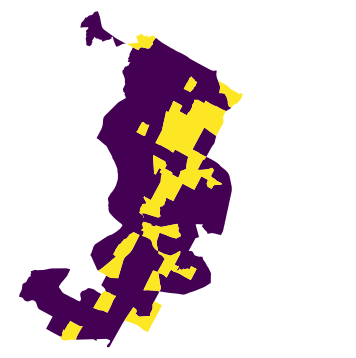
\includegraphics{./Figs/dissolve.png}
\end{frame}

\hypertarget{puna-me-projeksionet-e-hartave}{%
\section{Puna me Projeksionet e
Hartave}\label{puna-me-projeksionet-e-hartave}}

\begin{frame}{Puna me Projeksionet e Hartave}
\protect\hypertarget{puna-me-projeksionet-e-hartave-1}{}
\begin{itemize}
\tightlist
\item
  Sistemi i Referencës së Koordinatave (CRS) është një përkufizim
  matematikor që përcakton mënyrën se si koordinatat e gjeometrive
  lidhën me lokacionet e tyre reale në Tokë.
\end{itemize}
\end{frame}

\begin{frame}[fragile]{Puna me Projeksionet e Hartave}
\protect\hypertarget{puna-me-projeksionet-e-hartave-2}{}
CRS përbëhet nga disa pjesë kyçe:

\begin{verbatim}
**Datum**:
\end{verbatim}

Një datum është një model matematik që përcakton formën e Tokës dhe
përdoret për të përcaktuar origjinën dhe orientimin e një CRS.
\end{frame}

\begin{frame}{Puna me Projeksionet e Hartave}
\protect\hypertarget{puna-me-projeksionet-e-hartave-3}{}
Ekzistojnë dy lloje kryesore të datumeve:

\textbf{Horizontal:} Përcakton pozitën dhe formën e sipërfaqes së Tokës
në dy dimensione (gjerësia dhe gjatësia).

\textbf{Vertikal:} Përcakton nivelin bazë për lartësinë.
\end{frame}

\begin{frame}{Puna me Projeksionet e Hartave}
\protect\hypertarget{puna-me-projeksionet-e-hartave-4}{}
\textbf{Sistemi i Koordinatave:}

Ky sistem përcakton njësi matëse dhe boshtet (si latitudë dhe longitudë)
që përdoren për të vendosur gjeometri.
\end{frame}

\begin{frame}{Puna me Projeksionet e Hartave}
\protect\hypertarget{puna-me-projeksionet-e-hartave-5}{}
Dy llojet kryesore të sistemeve të koordinatave janë:

\textbf{Gjeografik (ellipsoidal):} Përdor një elipsoid për të përcaktuar
pozitën në një sipërfaqe me koordinata gradësh (gjerësia dhe gjatësia).

\textbf{Projektuar (planiometrik):} Projekton sipërfaqen e Tokës në një
plan të sheshtë duke përdorur një projeksion hartash dhe zakonisht
përdor njësi matëse lineare.
\end{frame}

\begin{frame}{Puna me Projeksionet e Hartave}
\protect\hypertarget{puna-me-projeksionet-e-hartave-6}{}
\textbf{Projeksioni i hartave:}

Një projeksion hartash është një transformim matematik që projekton
gjeometri nga një sipërfaqe elipsoidale në një sipërfaqe të sheshtë.
\end{frame}

\begin{frame}{Puna me Projeksionet e Hartave}
\protect\hypertarget{puna-me-projeksionet-e-hartave-7}{}
Disa lloje projeksionesh të zakonshme përfshijnë:

\textbf{Cilindrike:} Projekton globin në një formë cilindrike (si
Mercator).

\textbf{Koni:} Projekton globin në një kon.

\textbf{Azimutha:} Projekton globin në një rreth.
\end{frame}

\begin{frame}{Puna me Projeksionet e Hartave}
\protect\hypertarget{puna-me-projeksionet-e-hartave-8}{}
\textbf{Kodi EPSG}

Një kod EPSG është një numër unik që identifikon një CRS të caktuar.
Organizata EPSG mirëmban një bazë të dhënash me këta kode.
\end{frame}

\begin{frame}{Puna me Projeksionet e Hartave}
\protect\hypertarget{puna-me-projeksionet-e-hartave-9}{}
\textbf{Zona e Përdorimit (Area of Use):}

Përcakton rajonin gjeografik ku një CRS është i saktë dhe i përshtatshëm
për t'u përdorur.
\end{frame}

\begin{frame}{Puna me Projeksionet e Hartave}
\protect\hypertarget{puna-me-projeksionet-e-hartave-10}{}
\begin{itemize}
\item
  Mjeti ynë kryesor për menaxhimin e sistemeve të referencës së
  koordinatave është biblioteka \textbf{PROJ}, e cila mund të përdoret
  nëpërmjet bibliotekës \textbf{pyproj} të Python.
\item
  \textbf{Pyproj} mund të përdoret për të hyrë në informacionin CRS të
  një grupi të caktuar të dhënash gjeografike dhe gjithashtu për të
  riprojektuar të dhënat nga një sistem koordinatash në një tjetër.
\end{itemize}
\end{frame}

\begin{frame}[fragile]{Puna me Projeksionet e Hartave}
\protect\hypertarget{puna-me-projeksionet-e-hartave-11}{}
\begin{itemize}
\item
  Do shohim si të punojmë me sistemet e referencës së koordinatave në
  \texttt{geopandas} duke përdorur një grup të dhënash të kufijve të një
  vendi nga Evropa.
\item
  Do të riprojektojmë grupin e të dhënave nga sistemi origjinal WGS84 në
  një projeksion Lambert Azimuthal Equal Area, të cilin BE e rekomandon
  për Evropën
\end{itemize}
\end{frame}

\begin{frame}[fragile]{Puna me Projeksionet e Hartave}
\protect\hypertarget{puna-me-projeksionet-e-hartave-12}{}
\begin{itemize}
\item
  Fillojmë duke lexuar të dhënat nga skedari
  \texttt{eu\_countries\_2022.gpkg}.
\item
  Kur lexoni të dhënat në \texttt{GeoDataFrame} me \texttt{geopandas},
  informacioni CRS lexohet automatikisht nga skedari dhe ruhet në
  atributin \texttt{.crs}:
\end{itemize}
\end{frame}

\begin{frame}[fragile]{Puna me Projeksionet e Hartave}
\protect\hypertarget{puna-me-projeksionet-e-hartave-13}{}
\AddToHookNext{env/Highlighting/begin}{\scriptsize}

\begin{Shaded}
\begin{Highlighting}[]
\ImportTok{import}\NormalTok{ geopandas }\ImportTok{as}\NormalTok{ gpd}

\CommentTok{\# Lexo skedarin}
\NormalTok{fp }\OperatorTok{=} \StringTok{"data/gis2/EU\_countries/eu\_countries\_2022.gpkg"}
\NormalTok{data }\OperatorTok{=}\NormalTok{ gpd.read\_file(fp)}
\end{Highlighting}
\end{Shaded}
\end{frame}

\begin{frame}[fragile]{Puna me Projeksionet e Hartave}
\protect\hypertarget{puna-me-projeksionet-e-hartave-14}{}
\AddToHookNext{env/Highlighting/begin}{\scriptsize}

\begin{Shaded}
\begin{Highlighting}[]
\CommentTok{\# Cili është lloji?}
\BuiltInTok{print}\NormalTok{(}\BuiltInTok{type}\NormalTok{(data.crs))}
\CommentTok{\# Kontrollo informacionin e sistemit të referencës së koordinatave}
\NormalTok{data.crs}
\end{Highlighting}
\end{Shaded}
\end{frame}

\begin{frame}{Puna me Projeksionet e Hartave}
\protect\hypertarget{puna-me-projeksionet-e-hartave-15}{}
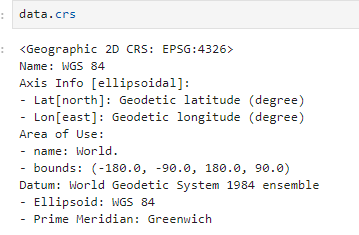
\includegraphics{./Figs/crs.png}
\end{frame}

\begin{frame}{Puna me Projeksionet e Hartave}
\protect\hypertarget{puna-me-projeksionet-e-hartave-16}{}
\begin{itemize}
\item
  Ajo që kthen \textbf{geopandas} këtu është në fakt një objekt
  \textbf{CRS} nga biblioteka \textbf{pyproj}.
\item
  Kodi \textbf{EPSG} i të dhënave tona është \textbf{4326} që i
  referohet sistemit të koordinatave \textbf{WGS84}.
\end{itemize}
\end{frame}

\begin{frame}{Puna me Projeksionet e Hartave}
\protect\hypertarget{puna-me-projeksionet-e-hartave-17}{}
\begin{itemize}
\item
  Ky kod EPSG është ndër më të përdorurit në botë për referencë
  gjeohapësinore.
\item
  Duke parë vlerat e koordinatave në kolonën geometry, ato janë në gradë
  dhjetore që përputhen me këtë sistem:
\end{itemize}
\end{frame}

\begin{frame}[fragile]{Puna me Projeksionet e Hartave}
\protect\hypertarget{puna-me-projeksionet-e-hartave-18}{}
\AddToHookNext{env/Highlighting/begin}{\scriptsize}

\begin{Shaded}
\begin{Highlighting}[]
\NormalTok{data[}\StringTok{"geometry"}\NormalTok{].head()}
\end{Highlighting}
\end{Shaded}
\end{frame}

\begin{frame}{Puna me Projeksionet e Hartave}
\protect\hypertarget{puna-me-projeksionet-e-hartave-19}{}
\begin{itemize}
\item
  Siç mund ta shohim, vlerat e koordinatave të Poligonit duken vërtet si
  shkallë dhjetore, kështu që gjithçka duket e saktë.
\item
  Megjithatë, \textbf{WGS84} nuk është një sistem koordinatash i mirë
  për të përfaqësuar kufijtë evropianë në një hartë, sepse sipërfaqet
  shtrembërohen.
\end{itemize}
\end{frame}

\begin{frame}{Puna me Projeksionet e Hartave}
\protect\hypertarget{puna-me-projeksionet-e-hartave-20}{}
\begin{itemize}
\tightlist
\item
  Prandaj, është një ide e mirë të konvertohen këto gjeometri në një
  projeksion \textbf{Lambert Azimuthal Equal Area {[}4{]} (EPSG:3035)},
  i cili është një opsion i mirë për krijimin e hartave me të dhëna në
  nivel shteti në Evropë.
\end{itemize}
\end{frame}

\begin{frame}[fragile]{Riprojektimi i një GeoDataFrame}
\protect\hypertarget{riprojektimi-i-njuxeb-geodataframe}{}
\begin{itemize}
\item
  Ndryshimi nga një sistem koordinatash në një tjetër është një nga
  detyrat më të zakonshme kur punojmë me të dhëna gjeografike.
\item
  Transformimi i koordinatave mund të bëhet shumë lehtë në
  \texttt{geopandas} duke përdorur metodën \texttt{.to\_crs()} të një
  \texttt{GeoDataFrame} të caktuar.
\end{itemize}
\end{frame}

\begin{frame}[fragile]{Riprojektimi i një GeoDataFrame}
\protect\hypertarget{riprojektimi-i-njuxeb-geodataframe-1}{}
Metoda ka dy parametra alternative:

\begin{itemize}
\item
  \texttt{crs} i cili pranon informacionin CRS nga formate të ndryshme,
  si vargjet \texttt{proj} ose teksti \texttt{OGS\ WKT};
\item
  \texttt{epgs} që pranon kodin EPSG të një sistemi të caktuar
  koordinatash si një numër.
\end{itemize}
\end{frame}

\begin{frame}[fragile]{Riprojektimi i një GeoDataFrame}
\protect\hypertarget{riprojektimi-i-njuxeb-geodataframe-2}{}
\begin{itemize}
\item
  Të dyja këto mund të përdoren për të bërë transformimin e koordinatave
  dhe për të riprojektuar të dhënat në një CRS të dëshiruar.
\item
  Le të riprojiktojmë të dhënat tona në EPSG:3035 duke përdorur
  parametrin \texttt{epsg}:
\end{itemize}
\end{frame}

\begin{frame}[fragile]{Riprojektimi i një GeoDataFrame}
\protect\hypertarget{riprojektimi-i-njuxeb-geodataframe-3}{}
\AddToHookNext{env/Highlighting/begin}{\scriptsize}

\begin{Shaded}
\begin{Highlighting}[]
\CommentTok{\# Le të bëjmë një kopje rezervë të të dhënave tona}
\NormalTok{data\_wgs84 }\OperatorTok{=}\NormalTok{ data.copy()}

\CommentTok{\# Riprojektimi i të dhënave}
\NormalTok{data }\OperatorTok{=}\NormalTok{ data.to\_crs(epsg}\OperatorTok{=}\DecValTok{3035}\NormalTok{)}

\CommentTok{\# Kontrollo vlerat e reja të gjeometrisë}
\NormalTok{data[}\StringTok{"geometry"}\NormalTok{].head()}
\end{Highlighting}
\end{Shaded}
\end{frame}

\begin{frame}[fragile]{Riprojektimi i një GeoDataFrame}
\protect\hypertarget{riprojektimi-i-njuxeb-geodataframe-4}{}
\AddToHookNext{env/Highlighting/begin}{\scriptsize}

\begin{Shaded}
\begin{Highlighting}[]
\CommentTok{\# Cili është kodi i ri EPSG?}
\NormalTok{data.crs.to\_epsg()}
\end{Highlighting}
\end{Shaded}
\end{frame}

\begin{frame}{Riprojektimi i një GeoDataFrame}
\protect\hypertarget{riprojektimi-i-njuxeb-geodataframe-5}{}
\begin{itemize}
\item
  Vlerat e koordinatave në gjeometri janë ndryshuar!
\item
  Tani kemi ndryshuar me sukses CRS-në e shtresës sonë në një të re,
  dmth. në sistemin e koordinatave planar ETRS-LAEA (EPSG:3035).
\end{itemize}
\end{frame}

\begin{frame}{Riprojektimi i një GeoDataFrame}
\protect\hypertarget{riprojektimi-i-njuxeb-geodataframe-6}{}
\begin{itemize}
\item
  Për të kuptuar vërtet se çfarë po ndodh, është mirë të eksploroni të
  dhënat tona vizualisht.
\item
  Le të krahasojmë grupet e të dhënave duke bërë harta prej tyre:
\end{itemize}
\end{frame}

\begin{frame}[fragile]{Riprojektimi i një GeoDataFrame}
\protect\hypertarget{riprojektimi-i-njuxeb-geodataframe-7}{}
\AddToHookNext{env/Highlighting/begin}{\scriptsize}

\begin{Shaded}
\begin{Highlighting}[]
\ImportTok{import}\NormalTok{ matplotlib.pyplot }\ImportTok{as}\NormalTok{ plt}

\CommentTok{\# Krijo nën{-}dritare të vendosura pranë njëra{-}tjetrës}
\NormalTok{fig, (ax1, ax2) }\OperatorTok{=}\NormalTok{ plt.subplots(nrows }\OperatorTok{=} \DecValTok{1}\NormalTok{, ncols }\OperatorTok{=} \DecValTok{2}\NormalTok{, figsize }\OperatorTok{=}\NormalTok{ (}\DecValTok{12}\NormalTok{, }\DecValTok{12}\NormalTok{))}

\CommentTok{\# Vizualizo të dhënat në CRS WGS84}
\NormalTok{data\_wgs84.plot(ax }\OperatorTok{=}\NormalTok{ ax1, facecolor }\OperatorTok{=} \StringTok{"gray"}\NormalTok{)}

\CommentTok{\# Shto titullin}
\NormalTok{ax1.set\_title(}\StringTok{"WGS84"}\NormalTok{)}

\CommentTok{\# Vizualizo të dhënat me projeksion ETRS{-}LAEA}
\NormalTok{data.plot(ax }\OperatorTok{=}\NormalTok{ ax2, facecolor }\OperatorTok{=} \StringTok{"blue"}\NormalTok{)}

\CommentTok{\# Shto titullin}
\NormalTok{ax2.set\_title(}\StringTok{"ETRS Lambert Azimuthal Equal Area projection"}\NormalTok{)}

\CommentTok{\# Vendos raportin si 1}
\NormalTok{ax1.set\_aspect(aspect }\OperatorTok{=} \DecValTok{1}\NormalTok{)}
\NormalTok{ax2.set\_aspect(aspect }\OperatorTok{=} \DecValTok{1}\NormalTok{)}

\CommentTok{\# Hiq hapësirën e bardhë të panevojshme rreth grafikut}
\NormalTok{plt.tight\_layout()}
\end{Highlighting}
\end{Shaded}
\end{frame}

\begin{frame}{Harta e Evropës e paraqitur me dy sisteme të ndryshme të
referencës së koordinatave}
\protect\hypertarget{harta-e-evropuxebs-e-paraqitur-me-dy-sisteme-tuxeb-ndryshme-tuxeb-referencuxebs-suxeb-koordinatave}{}
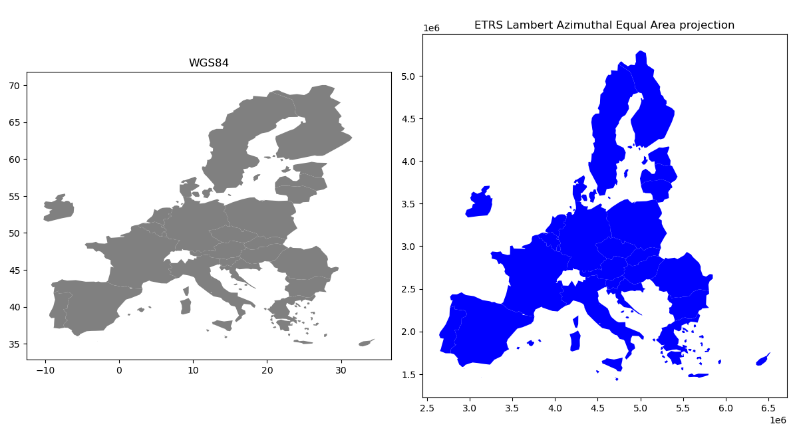
\includegraphics{./Figs/lambert.png}
\end{frame}

\begin{frame}{Harta e Evropës e paraqitur me dy sisteme të ndryshme të
referencës së koordinatave}
\protect\hypertarget{harta-e-evropuxebs-e-paraqitur-me-dy-sisteme-tuxeb-ndryshme-tuxeb-referencuxebs-suxeb-koordinatave-1}{}
\begin{itemize}
\tightlist
\item
  Siç mund të shohim nga figura, hartat duken shumë të ndryshme dhe ajo
  e riprojektuar duket dukshëm më mirë, veçanërisht në Veri, ku
  gjeometria është më realiste dhe jo aq e shtrirë sa në WGS84.
\end{itemize}
\end{frame}

\begin{frame}[fragile]{Harta e Evropës e paraqitur me dy sisteme të
ndryshme të referencës së koordinatave}
\protect\hypertarget{harta-e-evropuxebs-e-paraqitur-me-dy-sisteme-tuxeb-ndryshme-tuxeb-referencuxebs-suxeb-koordinatave-2}{}
\begin{itemize}
\tightlist
\item
  Së fundi, le të ruajmë shtresën tonë të projektuar në një Shapefile,
  në mënyrë që ta përdorim më vonë.
\end{itemize}

\AddToHookNext{env/Highlighting/begin}{\scriptsize}

\begin{Shaded}
\begin{Highlighting}[]
\CommentTok{\# Output}
\NormalTok{outfp }\OperatorTok{=} \StringTok{"data/temp/Europe\_borders\_epsg3035.shp"}

\CommentTok{\# Ruaj në disk}
\NormalTok{data.to\_file(outfp)  }
\end{Highlighting}
\end{Shaded}
\end{frame}

\end{document}
